% !TEX root = isae-beamer-template.tex

% Recall the outline at each section
\begin{frame}
  \frametitle{Definierter Zustand am Eingangspin}
	    \begin{column}{1\linewidth}
	    	Damit immer ein definierter Zustand am Eingang ist:
	    	\begin{center}
	    		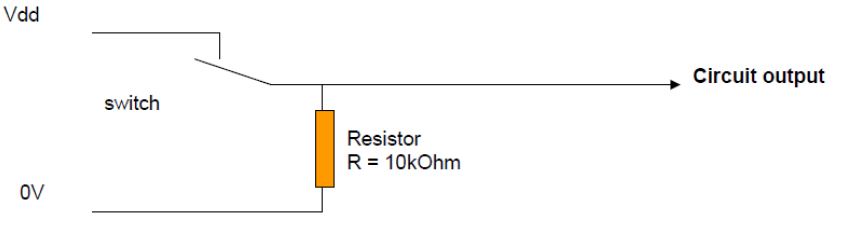
\includegraphics[width=1\textwidth]{images/Pullup.PNG}
	    	\end{center}
	    \end{column}
\end{frame}


\begin{frame}
	\frametitle{Definierter Zustand am Eingangspin}
	\begin{column}{1\linewidth}
		Externer oder interner Pull Widerstand benutzen.\\
		Bei Roboter V2, interne Pull Widerstände aktivieren.
		\begin{center}
			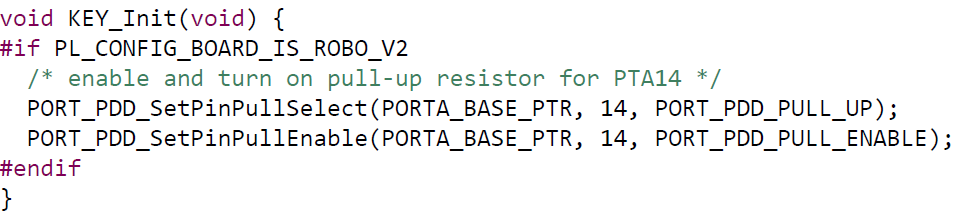
\includegraphics[width=1\textwidth]{images/ROBOV2.PNG}
		\end{center}
	\end{column}
\end{frame}

\begin{frame}
	\frametitle{Zustand einlesen, über Polling}
	\begin{column}{1\linewidth}
		Häufiges Abfragen der Tastereingänge.\\
		\begin{center}
			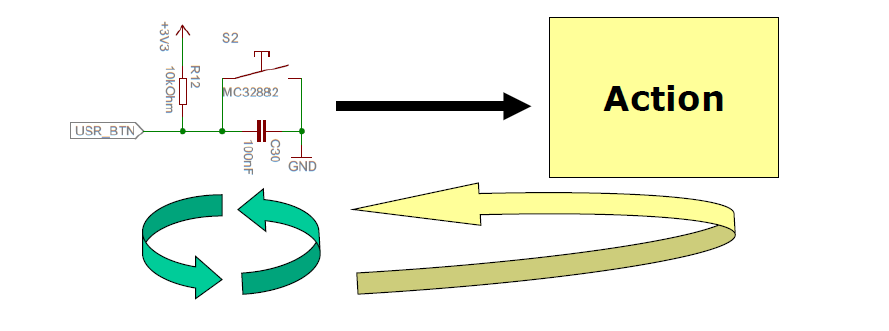
\includegraphics[width=1\textwidth]{images/Polling.PNG}
		\end{center}
	\end{column}
\end{frame}

\begin{frame}
	\frametitle{Zustand einlesen, über Interrupts}
	\begin{column}{1\linewidth}
		Kein Pollig, Interrupt bei Änderung.\\
		Pin muss Interrupt generieren können.
		\begin{center}
			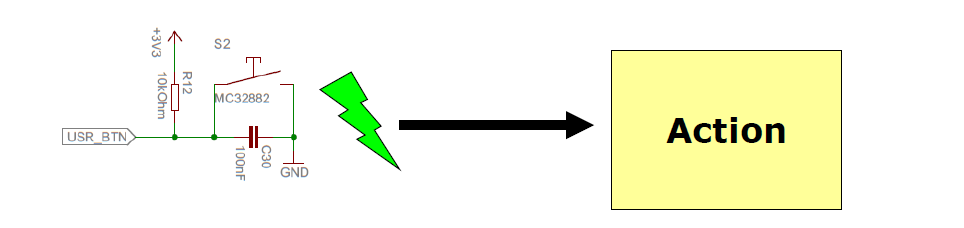
\includegraphics[width=1\textwidth]{images/Interrupt.PNG}
		\end{center}
	\end{column}
\end{frame}

\begin{frame}
	\frametitle{Ablauf mit Polling}
	\begin{column}{1\linewidth}
		\begin{center}
			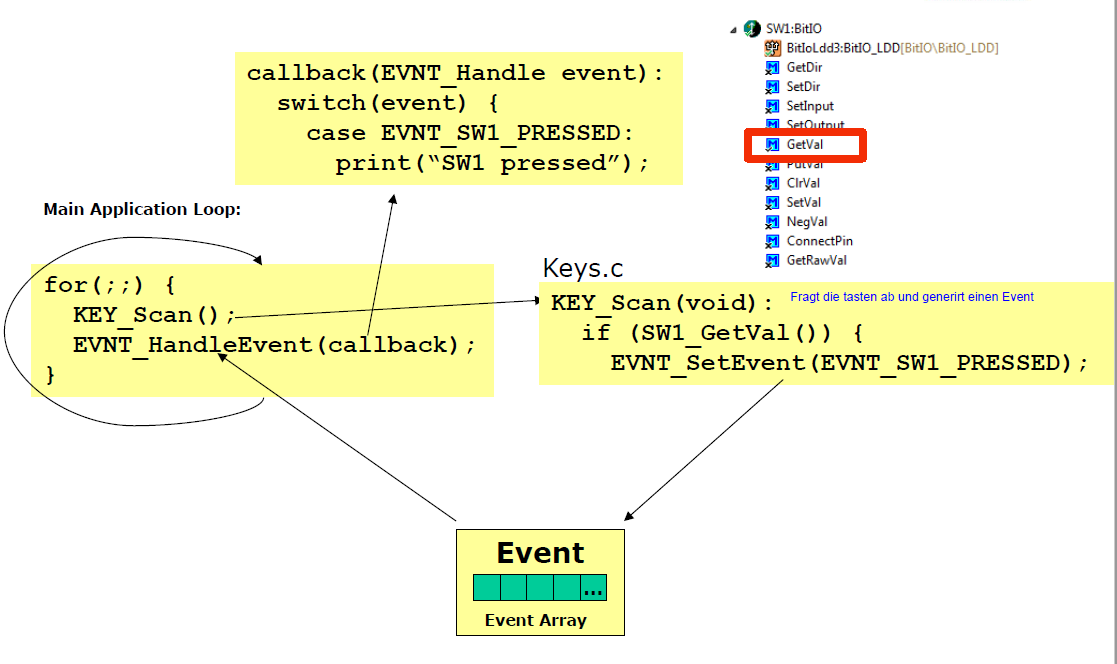
\includegraphics[width=1\textwidth]{images/Taster_Polling.PNG}
		\end{center}
	\end{column}
\end{frame}

\begin{frame}
	\frametitle{Ablauf mit Interrupts}
	\begin{column}{1\linewidth}
		\begin{center}
			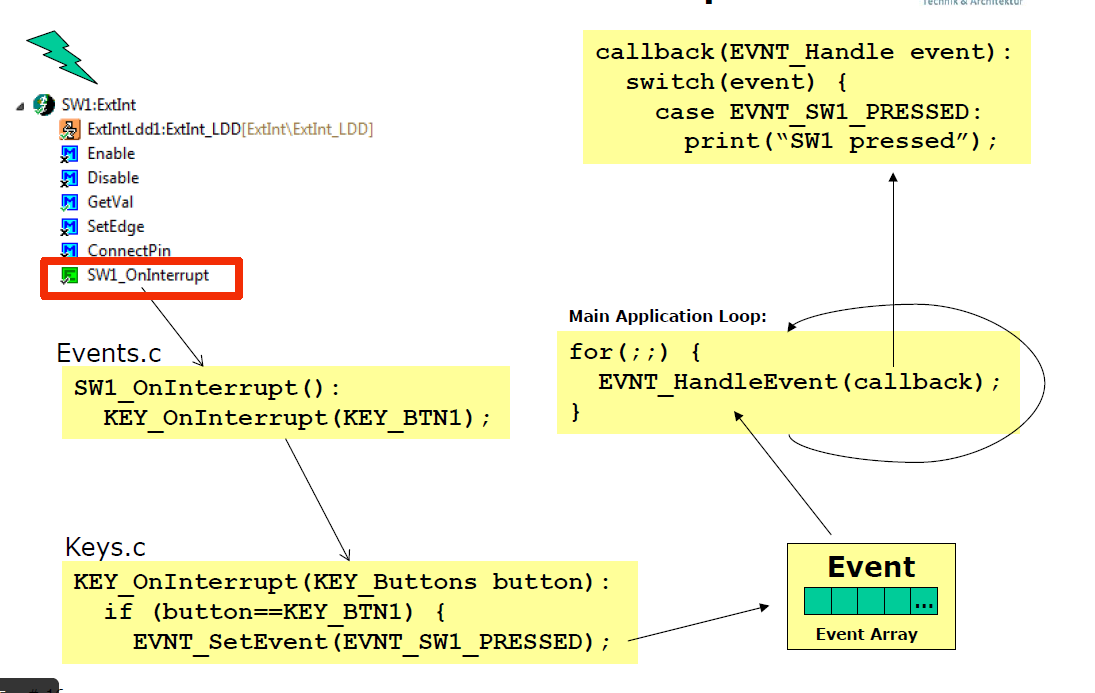
\includegraphics[width=1\textwidth]{images/Intrerrupt_Routine.PNG}
		\end{center}
	\end{column}
\end{frame}